
\begin{frame}{Learning Movement Primitives for the Humanoid Robot HRP2}
  \begin{itemize}
    \item Observation : Human movements are not feasible on humanoid robot.
  \end{itemize}
  \begin{center}
    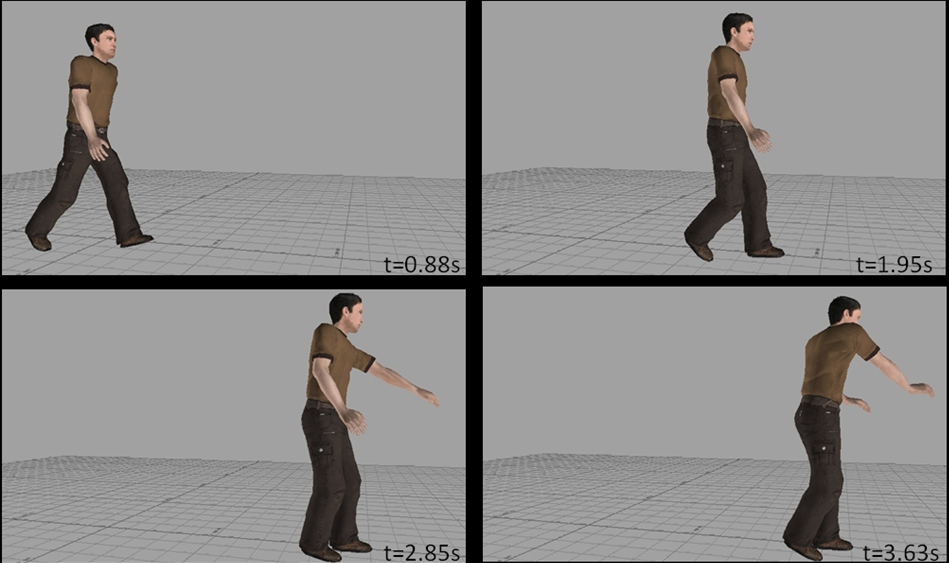
\includegraphics[height=0.4\textheight, keepaspectratio]
      {motion_primitives/realavatar.jpg}
    \hspace*{0.5cm}
    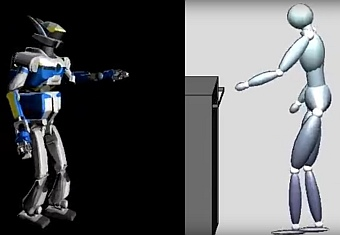
\includegraphics[height=0.4\textheight, keepaspectratio]
      {motion_primitives/RobotAvatarjpg2.jpg}
  \end{center}
  \begin{itemize}
    \item Hypothesis : Using MPC to ensure feasibility + human motion primitives should produce feasible whole body motions  
  \end{itemize}
\end{frame}

\begin{frame}{Implementation on HRP-2}
  %\vspace*{-0.8cm}  
  \begin{center}
    \tikzstyle{block} = [draw=black, fill=white, rectangle,
      minimum height=2em, minimum width=5em, align=center]
    \tikzstyle{point} = [coordinate]
    \tikzstyle{pinstyle} = [pin edge={to-,thin,black}]
    \begin{tikzpicture}
      \node [block, fill=white] at (0.0,0.0) (scheme) {
        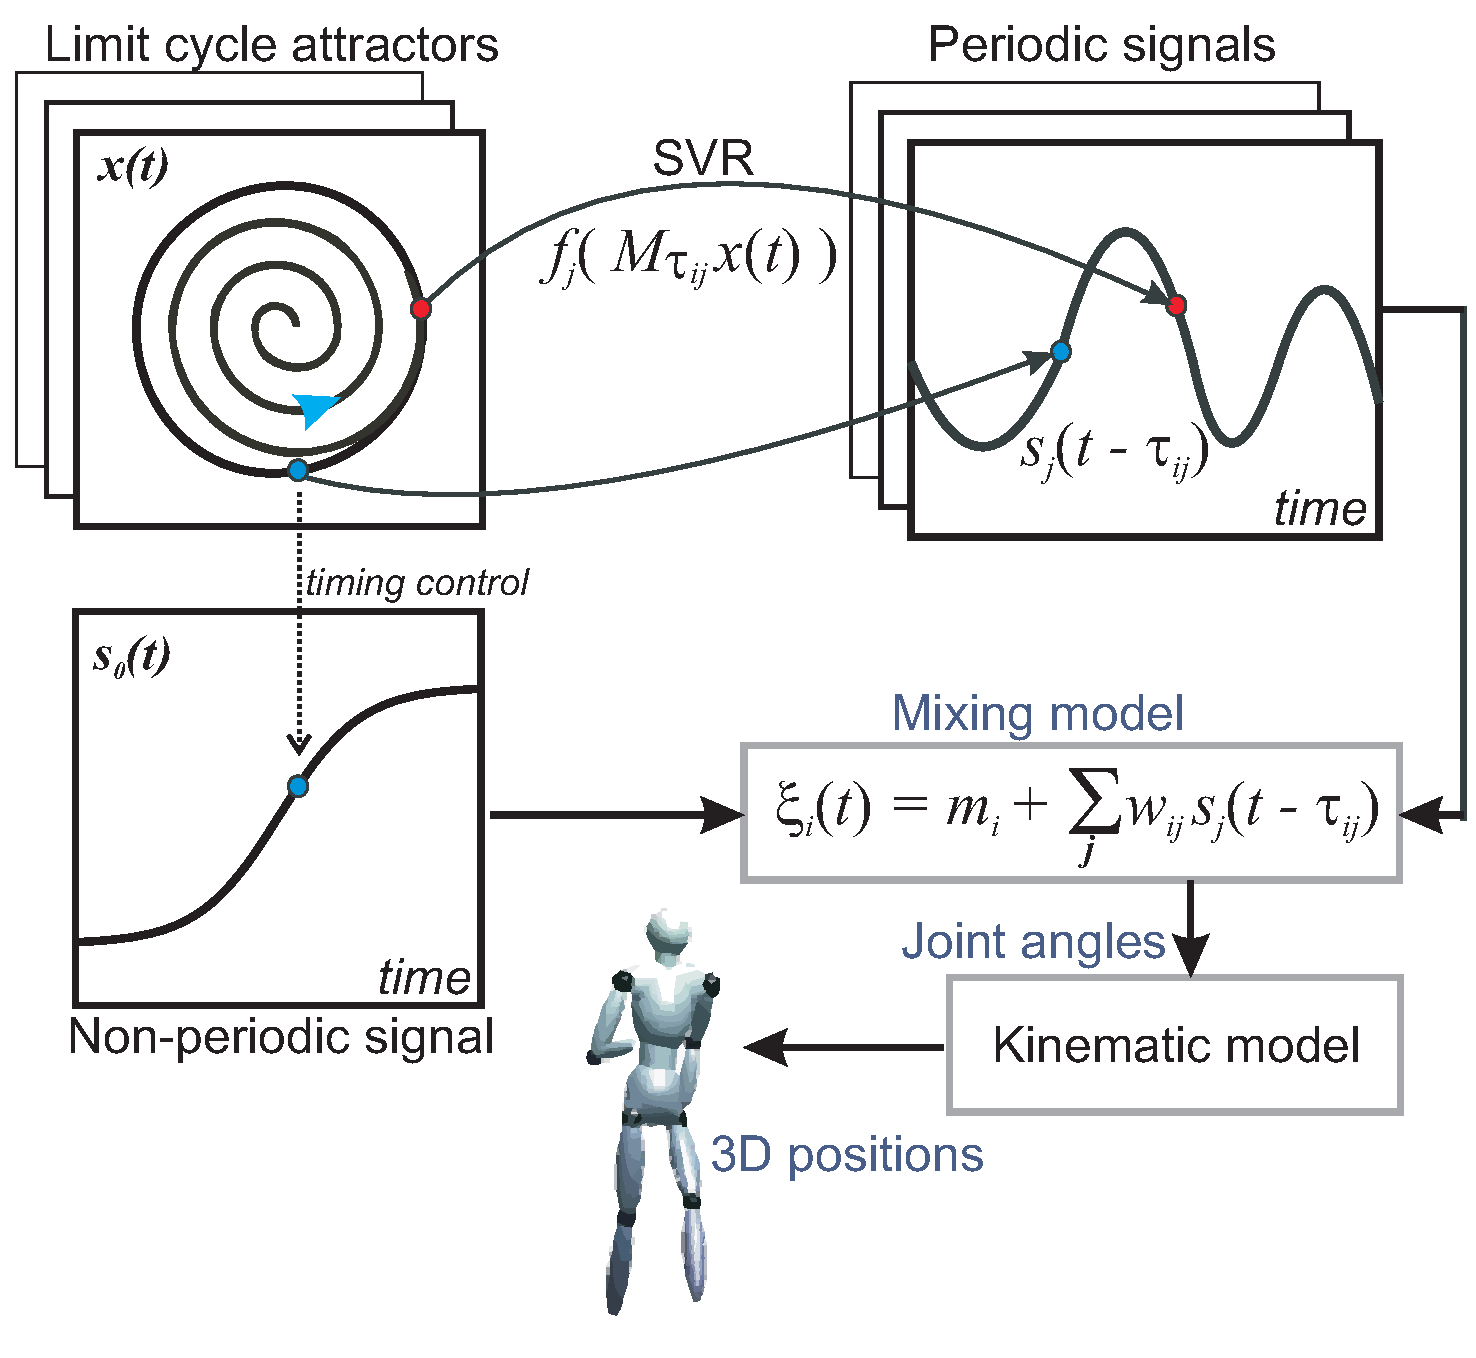
\includegraphics
        [height=0.4\textheight, keepaspectratio, trim={0.0cm 2.0cm 0.0cm 0.0cm},clip]
        {motion_primitives/Graph_syst.pdf}
        %trim={<left> <lower> <right> <upper>}
      };
%%%%
	    \node [block,  minimum width=0.1cm] at (0.0,2.5) (wpg) {
	        Walking Pattern Generator
	    };
%%%%
	    \node [block,  minimum width=0.1cm] at (5.0,1.5) (dyn) {
	        Dynamic Filter
	    };
%%%%%
      \draw [ - ] (scheme) -| node {} ([xshift=-1cm,yshift=-0.3cm]dyn.west);
      \draw [ ->] ([xshift=-1cm,yshift=-0.3cm]dyn.west) -- node {} ([yshift=-0.3cm]dyn.west);
      \draw [ - ] (wpg) -| node {} ([xshift=-1cm,yshift=+0.3cm]dyn.west);    
      \draw [ ->] ([xshift=-1cm,yshift=+0.3cm]dyn.west) -- node {} ([yshift=+0.3cm]dyn.west);      
    \end{tikzpicture}
    \begin{itemize}
      \item The upper body is learned from humans.
      \item The lower body is computed via MPC.
      \item The Dynamic Filter links them.
    \end{itemize}
  \end{center}
\end{frame}

\begin{frame}{Motion on HRP-2}
  \begin{center}
    \movie[autostart,loop]{
    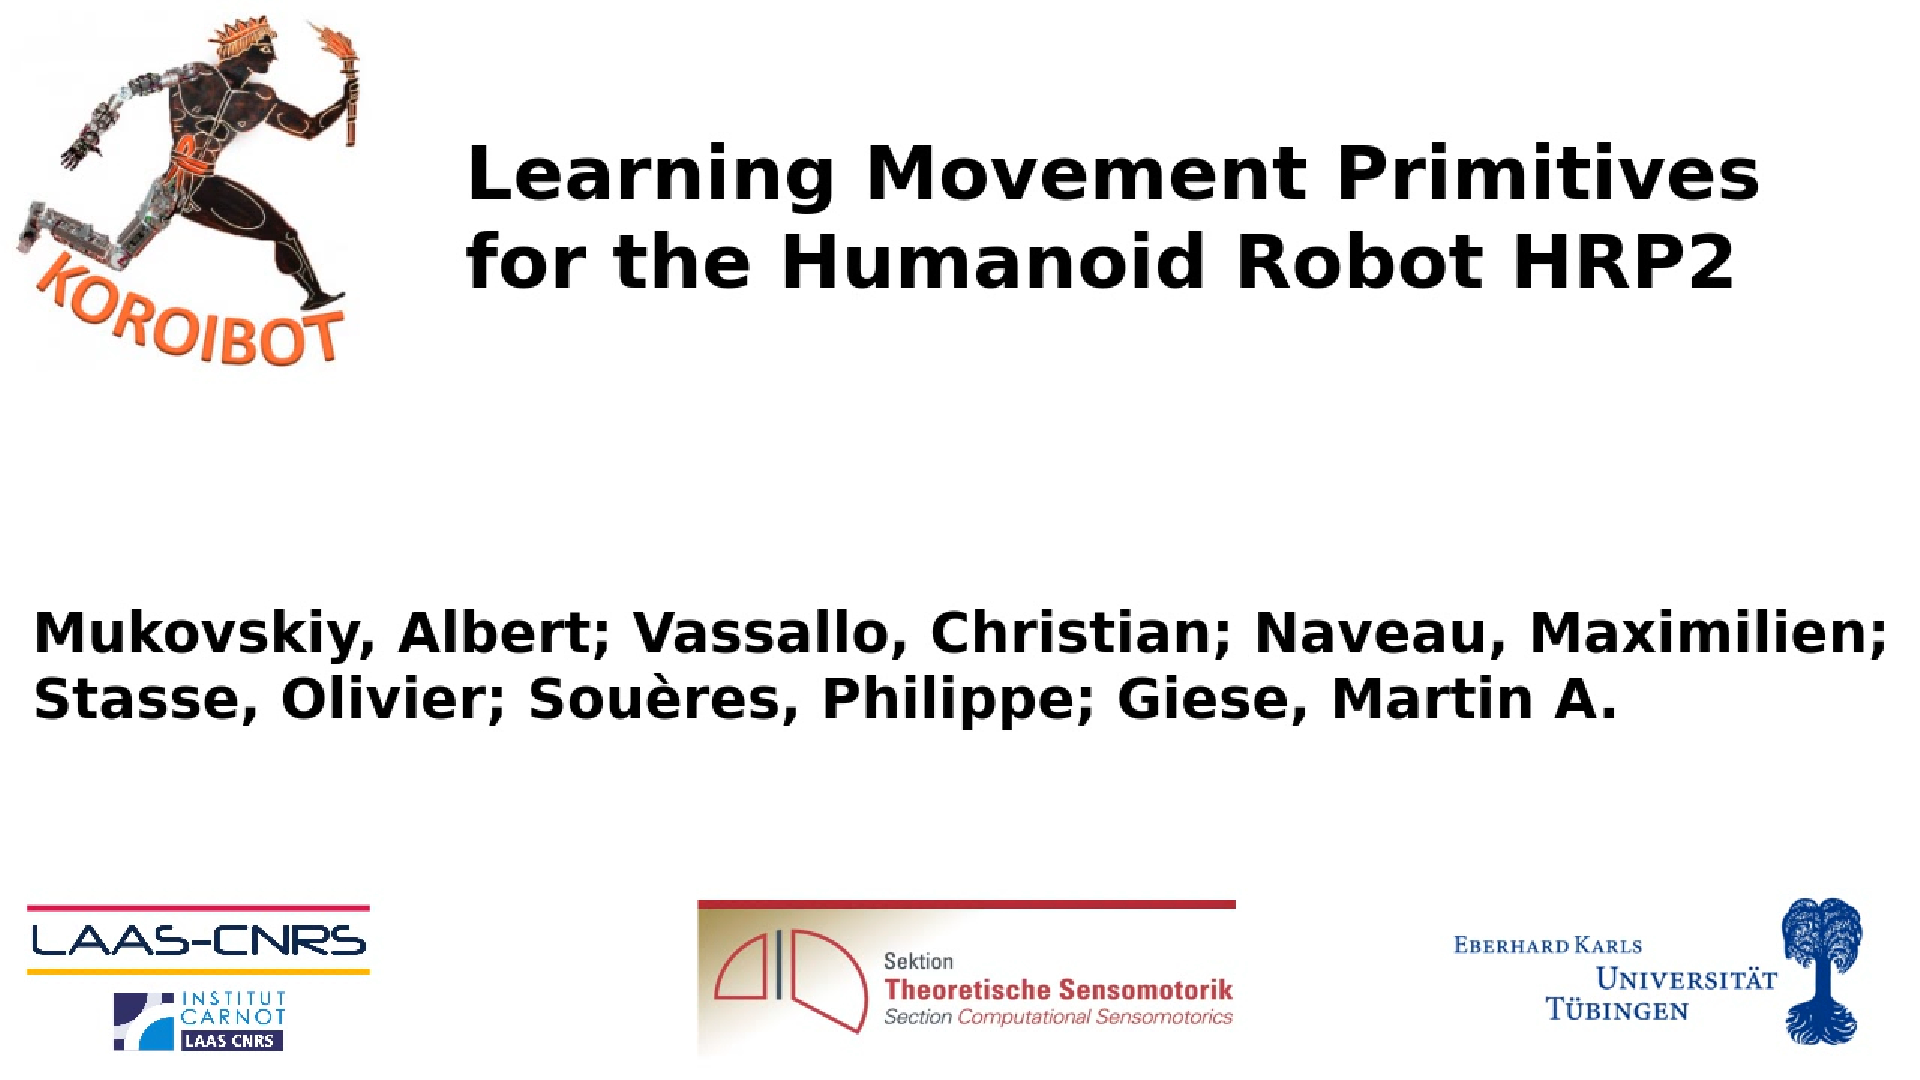
\includegraphics[width=0.9\linewidth, keepaspectratio]
      {motion_primitives/16-mukovskiy-elsarticle.png}    
    }  
    {./videos/16-mukovskiy-elsarticle-short.mp4}
  \end{center}
  \vspace*{-0.5cm}
  \blfootnote{Mukovskiy, Vassallo, \textbf{Naveau} et al. JRAS 2016}
\end{frame}


